% !TEX program = xelatex
\documentclass{article}
\usepackage{/Users/jay/LaTeX/cs}
\usepackage{/Users/jay/LaTeX/xeCJK}

\newcommand{\hmwkClass}{Probability and Statistics, Spring 2018}
\newcommand{\hmwkTitle}{Homework 6}
\newcommand{\hmwkDueDate}{June 11, 2018}
\newcommand{\tb}{\textbf}

\begin{document}

\thispagestyle{empty}
\section*{\hmwkClass \\
    \normalsize{\hmwkTitle} \\
    \normalsize{DUE DATE: \hmwkDueDate}
}

\hfill{B03902129 \, 資工四 \, 陳鵬宇}

\begin{enumerate}
    \item [7.1.2]

    The PMF of $X$ is

    $\text P_X(x) = \text P[X = x] = \begin{cases}
        \frac{1}{6} & x = 0, 1, \dots, 5 \\
        0           & \text{otherwise}.
    \end{cases}
    $

    $\text E[X] = \frac{0 + 5}{2} = 2.5$.

    \begin{align*}
        \text E[X \mid X \ge \text E[X]]
        & = \text E[X \mid X \ge \frac{5}{2}] \\
        & = \frac{3 + 4 + 5}{3} = 4.
    \end{align*}    

    \item [7.1.7]

    \begin{enumerate}[label=(\alph*)]
        \item Given that a person is healthy, the conditional PDF of Gaussian($\mu = 90$, $\sigma = 20$) random variable is

        \begin{align*}
            f_{X \mid H(x)}
            & = \frac{1}{\sqrt{2\pi\sigma^2}} e^{-(x - \mu)^2 / 2\sigma^2} \\
            & = \frac{1}{\sqrt{2\pi 400}} e^{-(x - 90)^2 / 800} \\
            & = \frac{1}{20\sqrt{2\pi}} e^{-(x - 90)^2 / 800}.
        \end{align*}

        \item 

        \begin{align*}
            \text P[T^+ \mid H]
            & = \text P[x \ge 140 \mid H] \\
            & = \text P \Big[\frac{X - \mu}{\sigma} \ge \frac{140 - \mu}{\sigma} \mid H \Big] \\
            & = \text P \Big[\frac{X - 90}{20} \ge \frac{140 - 90}{20} \Big] \\
            & = \text P \Big[\frac{X - 90}{20} \ge 2.5 \Big] \\
            & = \text P[Z \ge 2.5] \\
            & = 1 - \text P[Z \le 2.6] \\
            & = 1 - \Phi(2.5) \\
            & \approx 1 - 0.99379 \\
            & = 0.00621.
        \end{align*}

        \begin{align*}
            \text P[T^- \mid H]
            & = \text P[x \le 110 \mid H] \\
            & = \text P \Big[\frac{X - \mu}{\sigma} \le \frac{110 - \mu}{\sigma} \mid H \Big] \\
            & = \text P \Big[\frac{X - 90}{20} \le \frac{110 - 90}{20}] \\
            & = \text P[Z \le 1] \\
            & = \Phi(1) \\
            & = 0.8413.
        \end{align*}
       
        \item 
        $\text P[H \mid T^-] = \frac{\text P[H] \cdot \text P[T^- \mid H]}{\text P[T^-]}$

        where $\text P[T^-] = \text P[D] \cdot \text P[T^- \mid D] + \text P[H] \cdot \text P[T^- \mid H].$

        \begin{align*}
            P[T^- \mid D]
            & = \text P[x \le 110 \mid D] \\
            & = \text P \Big[\frac{X - \mu}{\sigma} \le \frac{110 - \mu}{\sigma} \mid D \Big] \\
            & = \text P \Big[\frac{X - 60}{40} \le \frac{110 - 60}{40}] \\
            & = \text P[Z \le 1.25] \\
            & = \Phi(1.25) \\
            & = 0.8944.
        \end{align*}

        \begin{align*}
            \text P[H \mid T^-]
            & = \frac{0.9 \cdot 0.8413}{(0.1 \cdot 0.8944) + (0.9 \cdot 0.8413)} \approx 0.8943.
        \end{align*}

        \item 
        Let
        \begin{align*}
            q 
            & = \text P[T^0 \mid H] \\
            & = 1 - \text P[T^- \mid H] - \text P[T^+ \mid H] \\
            & = 1 - 0.8413 - 0.0062 = 0.1525.
        \end{align*}

        $p = 1 - q = 1 - 0.1525 = 0.8475.$

        We have

        $P_{N \mid H}(n) = \begin{cases}
            (1 - p)^{n - 1}p & n = 1, 2, \dots, \\
            0 & \text{otherwise}.
        \end{cases}
        $
    \end{enumerate}

    \item [7.2.6]

    \begin{enumerate}[label=(\alph*)]
        \item 
        \begin{align*}
        \text P[\text{be sent to } A] 
        & = \text P[X = 2] + \text P[X = 4] + \text P[X = 6] + \text P[X = 8] \\
        & = 0.15 + 0.15 + 0.1 + 0.1 = 0.5.
        \end{align*}

        $$P_{X \mid A}(x) =
        \begin{cases}
            \frac{0.15}{0.5} = 0.3 & x = 2, 4, \\
            \frac{0.1}{0.5} = 0.2 & x = 6, 8, \\
            0 & \text{otherwise}.
        \end{cases}
        $$

        \begin{align*}
            \text E[X \mid A]
            & = \sum_{x = 2, 4, 6, 8} x \cdot P_{X \mid A}(x) \\
            & = (2 \cdot 0.3) + (4 \cdot 0.3) + (6 \cdot 0.2) + (8 \cdot 0.2) \\
            & = 0.6 + 1.2 + 1.2 + 1.6 = 4.6.
        \end{align*}

        \begin{align*}
            \text E[X^2 \mid A]
            & = \sum_{x = 2, 4, 6, 8} x^2 \cdot P_{X \mid A}(x) \\
            & = (2^2 \cdot 0.3) + (4^2 \cdot 0.3) + (6^2 \cdot 0.2) + (8^2 \cdot 0.2) \\
            & = 1.2 + 4.8 + 7.2 + 12.8 = 26.
        \end{align*}

        \begin{align*}
            \text{Var}[X \mid A]
            & = \text E[X^2 \mid A] - (\text E[X \mid A])^2 \\
            & = 26 - 4.6^2 \\
            & = 26 - 21.16 = 4.84.
        \end{align*}

        $\sigma_{X \mid A} = \sqrt{4.84} = 2.2.$
        
        \item
        \begin{align*}
            \text P[\text{be sent to } B \text{ and } \le 6] 
            & = \text P[X = 1] + \text P[X = 3] + \text P[X = 5] \\
            & = 0.15 + 0.15 + 0.1 = 0.4.
        \end{align*}

        $$P_{X \mid B}(x) =
        \begin{cases}
            \frac{0.15}{0.4} = 0.375 & x = 1, 3, \\
            \frac{0.1}{0.4} = 0.25 & x = 5, \\
            0 & \text{otherwise}.
        \end{cases}
        $$

        \begin{align*}
            \text E[X \mid B]
            & = \sum_{x = 1, 3, 5} x \cdot P_{X \mid A}(x) \\
            & = (1 \cdot 0.375) + (3 \cdot 0.375) + (5 \cdot 0.25) \\
            & = 0.375 + 1.125 + 1.25 = 2.75.
        \end{align*}

        \begin{align*}
            \text E[X^2 \mid B]
            & = \sum_{x = 1, 3, 5} x^2 \cdot P_{X \mid A}(x) \\
            & = (1^2 \cdot 0.375) + (3^2 \cdot 0.375) + (5^2 \cdot 0.25) \\
            & = 0.375 + 3.375 + 6.25 = 10.
        \end{align*}

        \begin{align*}
            \text{Var}[X \mid B]
            & = \text E[X^2 \mid B] - (\text E[X \mid B])^2 \\
            & = 10 - 2.75^2 \\
            & = 10 - 7.5625 = 2.4375.
        \end{align*}

        $\sigma_{X \mid B} = \sqrt{2.4375} \approx 1.56.$

    \end{enumerate}

    \item [7.3.5]

    \begin{enumerate}[label=(\alph*)]
        \item 
        \begin{align*}
            \text P[A]
            & = \text P[Y \le 1] \\
            & = \int_0^1 \int_0^1 f_{X, Y}(x, y) dy dx \\
            & = \int_0^1 \int_0^1 \frac{x + y}{3} dy dx \\
            & = \frac{1}{3}.
        \end{align*}

        \item 
        $$
        f_{X, Y \mid A}(x, y) = \begin{cases}
            \frac{f_{X, Y}(x, y)}{\text P[A]} = \frac{(x + y) / 3}{1 / 3} = (x + y) & 0 \le x \le 1; 0 \le y \le 1, \\
            0 & \text{otherwise}.
        \end{cases}
        $$

        \item
        \begin{align*}
            f_{X \mid A}(x)
            & = \int_0^1 f_{X, Y \mid A}(x, y) dy \\
            & = \int_0^1 (x + y) dy \\
            & = x + \frac{1}{2}.
        \end{align*}

        Thus,

        $$
        f_{X \mid A}(x) = \begin{cases}
            x + \frac{1}{2} & 0 \le x \le 1, \\
            0 & \text{otherwise}.
        \end{cases}
        $$

        \begin{align*}
            f_{Y \mid A}(y)
            & = \int_0^1 f_{X, Y \mid A}(x, y) dx \\
            & = \int_0^1 (x + y) dx \\
            & = y + \frac{1}{2}.
        \end{align*}

        Thus,

        $$
        f_{X \mid A}(y) = \begin{cases}
            y + \frac{1}{2} & 0 \le y \le 1, \\
            0 & \text{otherwise}.
        \end{cases}
        $$
    \end{enumerate}

    \item [7.4.10]

    \begin{enumerate}[label=(\alph*)]
        \item

        $X$ and $Y$ are independent if
        $$P_{X, Y}(x, y) = P_X(x) \cdot P_Y(y).$$
        
        $$
        \begin{array}{c|ccc|c}
            \text P_{X, Y}(x, y) & y = -1 & y = 0 & y = 1 & \text P_X(x) \\
            \hline
            x = -1 & 3 / 16 & 1 / 16 & 0     & \text P_X(-1) = 1 / 4 \\
            x = 0  & 1 / 6  & 1 / 6  & 1 / 6 & \text P_X(0) = 1 / 2 \\
            x = 1  & 0      & 1 / 8  & 1 / 8 & \text P_X(1) = 1 / 4 \\
            \hline
            \text P_Y(y) & \text P_Y(-1) = 17 / 48 & \text P_Y(0) = 17 / 48 & \text P_Y(1) = 14 / 48
        \end{array}
        $$

        $P_{X, Y}(-1, 1) = 0 \ne P_X(-1) \cdot P_Y(1) = \frac{1}{4} \cdot \frac{14}{48}.$

        Hence, $X$ and $Y$ are not independent.

        \item
        
        $ $ \\
        
        \begin{center}
        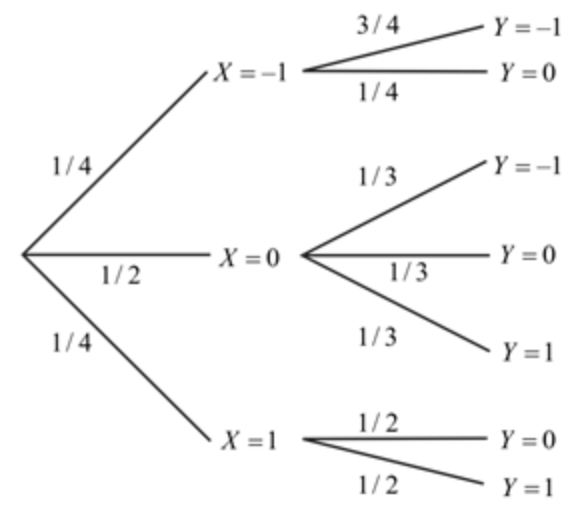
\includegraphics[width=0.3\textwidth]{img/7.4.10.png}
        \end{center}

    \end{enumerate}
\end{enumerate}

\end{document}